\chapter{Methodology}

This chapter formalizes our approach: the A* search procedure over reasoning traces, the heuristic design, the 13 topology features, and the routing strategies.

\section{Problem Formulation}

Let $\mathcal{Q} = (q, C, \mathcal{O})$ denote a reasoning problem, where $q$ is the question, $C$ is an optional context passage, and $\mathcal{O} = \{o_1, \ldots, o_K\}$ is the candidate answer set. A \emph{reasoning trace} $\tau = (s_1, s_2, \ldots, s_T)$ is an ordered sequence of natural-language reasoning steps, and a prediction function $\phi(\tau) \in \mathcal{O}$ extracts the final answer. Let $\mathcal{M}_\theta$ denote a language model with parameters $\theta$.

\section{Chain-of-Thought (CoT) Reasoning}

In CoT prompting, the model generates a single reasoning trace autoregressively:
\begin{equation}
s_t \sim \mathcal{M}_\theta(\cdot \mid q, C, \mathcal{O}, s_{1:t-1})
\end{equation}
Generation terminates when the model emits a terminal answer pattern, and the final prediction is $\hat{y}^{\text{CoT}} = \phi(\tau^{\text{CoT}})$. CoT explores exactly one element of the trace space with no mechanism for backtracking or branch comparison.

\section{A* Search over Reasoning Traces}

We search over the space of reasoning traces using an A*-style priority rule, with a finite node budget and a multi-goal voting procedure for tractability.

\subsection{State Space}

The search space is a tree $\mathcal{G} = (\mathcal{S}, \mathcal{E})$ where each node $n \in \mathcal{S}$ represents a partial reasoning state:
\begin{equation}
n = (\tau_n, d_n), \qquad \tau_n = (s_1, \ldots, s_{d_n})
\end{equation}
Here $\tau_n$ is the partial trace at node $n$ and $d_n = |\tau_n|$ is its depth. The root node $n_0$ has $\tau_{n_0} = \emptyset$ and $d_{n_0} = 0$.

\subsection{Successor Generation}

Given a node $n$, we ask the language model to propose $N_c$ candidate next steps:
\begin{equation}
\{(s^{(j)}, c^{(j)})\}_{j=1}^{N_c} = \texttt{GenerateSteps}(\mathcal{M}_\theta, q, C, \mathcal{O}, \tau_n, N_c)
\end{equation}
Each candidate consists of step text $s^{(j)}$ and a self-reported confidence $c^{(j)} \in [0.0, 1.0]$.

\subsection{Goal Condition}

A node is a goal node if its last step contains a terminal answer pattern:
\begin{equation}
\texttt{IsGoal}(n) = \mathds{1}\Big[\exists p \in \mathcal{P}: p \subset s_{d_n}\Big]
\end{equation}
where $\mathcal{P}$ contains answer templates such as ``The answer is [A/B/C/D]'' for multiple-choice tasks.

\subsection{Path Cost}

The cumulative cost trades off reasoning length and uncertainty:
\begin{equation}
g(n) = \sum_{t=1}^{d_n} \big[1 + (1-c_t)\big] = d_n + \sum_{t=1}^{d_n}(1-c_t)
\end{equation}
Each step contributes a base cost of 1, and lower-confidence steps incur additional penalty.

\subsection{Priority Function}

Nodes are expanded in order of $f(n) = g(n) + h(n)$, where $h(n)$ is the heuristic estimate of remaining cost to a goal.

\section{Heuristic Design}

\subsection{Depth-Coverage Heuristic}

The heuristic combines depth and entity coverage:
\begin{equation}
h(n) = \omega_d \max(0, H_{\min} - d_n) + \omega_c(1 - E(n))
\end{equation}
where $H_{\min}$ is a task-level lower bound on required reasoning hops, $E(n) \in [0,1]$ is the fraction of target entities covered by the partial trace, and $\omega_d, \omega_c > 0$ are weights.

\subsection{Entity Coverage Computation}

For a question $q$, we extract content units $\mathcal{E}_q$ consisting of quoted strings, proper-name phrases, numbers, and non-stopword content terms. Coverage is:
\begin{equation}
E(n) = \frac{|\{e \in \mathcal{E}_q : e \text{ appears in } \tau_n\}|}{|\mathcal{E}_q|}
\end{equation}

\subsection{Admissibility}

\begin{theorem}[Conservative Admissibility]
Under the minimum-hop assumption and non-goal continuation assumption, if $\omega_d + \omega_c \leq c_{\min} = 1 + (1 - c_{\max})$, then $h(n) \leq h^*(n)$ for all non-goal nodes.
\end{theorem}

In our implementation, $H_{\min} = 2$, $\omega_d = \omega_c = 0.3$, and $c_{\max} = 0.99$, giving $c_{\min} = 1.01 > \omega_d + \omega_c = 0.6$, satisfying admissibility.

\subsection{Human Validation}

We validated the heuristic against human progress judgments on 500 partial states. The heuristic underestimates progress on average (0.43 vs. human 0.58, paired $t$-test $p < 0.001$), with overestimation rate 12.3\% and maximum overestimation $\epsilon_{\max} = 0.14$. This confirms conservative behavior.

\section{The A* Algorithm}

Algorithm~\ref{alg:astar_thesis} presents the complete procedure.

\begin{algorithm}[ht]
\caption{Budgeted A* Search over Reasoning Traces}
\label{alg:astar_thesis}
\begin{algorithmic}[1]
\REQUIRE Problem $\mathcal{Q} = (q, C, \mathcal{O})$, model $\mathcal{M}_\theta$, depth limit $D_{\max}$, node budget $B$, candidates $N_c$
\STATE Initialize root $n_0 \gets (\emptyset, 0)$, $g(n_0) \gets 0$
\STATE $\texttt{Open} \gets \{n_0\}$ (priority queue on $f(n) = g(n) + h(n)$)
\STATE $\texttt{Goals} \gets \emptyset$, explored $\gets 0$
\WHILE{$\texttt{Open} \neq \emptyset$ and explored $< B$}
    \STATE $n \gets \texttt{Open}.\text{pop\_min}()$
    \STATE explored $\gets$ explored $+ 1$
    \IF{$\texttt{IsGoal}(n)$}
        \STATE $\texttt{Goals} \gets \texttt{Goals} \cup \{n\}$; continue
    \ENDIF
    \IF{$d_n \geq D_{\max}$}
        \STATE continue
    \ENDIF
    \STATE $\{(s^{(j)}, c^{(j)})\}_{j=1}^{N_c} \gets \texttt{GenerateSteps}(\mathcal{M}_\theta, q, C, \mathcal{O}, \tau_n, N_c)$
    \FOR{each $(s^{(j)}, c^{(j)})$}
        \STATE $n' \gets (\tau_n \oplus s^{(j)}, d_n + 1)$
        \STATE $g(n') \gets g(n) + 1 + (1 - c^{(j)})$
        \STATE $\texttt{Open}.\text{push}(n', g(n') + h(n'))$
    \ENDFOR
\ENDWHILE
\RETURN weighted vote over $\texttt{Goals}$
\end{algorithmic}
\end{algorithm}

\section{Routing Strategies}

Given the complementarity between CoT and A*, we define routing functions $\mathcal{R}: \mathcal{Q} \to \{\text{CoT}, A^*\}$. We distinguish two families.

\subsection{Output-Based Routers (Post-Generation)}

These require generating traces before deciding:

\textbf{Semantic Entropy:} Generate $N=5$ CoT samples, compute answer disagreement. If $\geq 3$ unique answers, route to A* (high uncertainty suggests search helps).

\textbf{LLM-as-Critic:} Generate both CoT and A* traces, ask a critic model (DeepSeek-R1-Distill-Qwen-14B) to diagnose flaws in each and select the better trace.

\textbf{LLM-as-Judge:} Similar to critic but verdict-oriented---the judge compares both traces on faithfulness and logical validity, returning only the winner.

\subsection{Pre-Generation Routers}

These decide before any generation:

\textbf{Random Forest:} Trained on hand-crafted features (question length, connectives, negation) using 5-fold stratified cross-validation.

\textbf{Topology Router:} XGBoost/GradientBoosting classifier on the 13 topology features described below. Requires no LLM inference at routing time.

\section{Reasoning Topology Features}
\label{sec:topology_features}

We define 13 pre-generation features computed directly from the input text:

\begin{enumerate}
\item \textbf{q\_len:} Question length (word count)
\item \textbf{ctx\_len:} Context length (word count)
\item \textbf{conn\_count:} Logical connectives (if, then, because, since, although, however, but, unless, either, neither, both, all, some, none, etc.)
\item \textbf{neg\_count:} Negation markers (not, no, never, nothing, without, impossible, cannot, etc.)
\item \textbf{hop\_count:} Multi-hop indicators (who, which, where, what, when, related to, associated with, caused by, led to, etc.)
\item \textbf{cmp\_count:} Comparison words (more, less, greater, fewer, larger, smaller, better, worse, than, etc.)
\item \textbf{q\_marks:} Number of question marks (sub-questions)
\item \textbf{ctx\_sents:} Number of sentences in context
\item \textbf{concept\_count:} Unique named entities (capitalized multi-letter words)
\item \textbf{linearity\_score:} $1 / (1 + \text{branching\_signals})$ --- inverse of branching complexity
\item \textbf{n\_options:} Number of answer options (for multiple-choice)
\item \textbf{depth\_est:} Estimated reasoning depth $= \text{hop\_count} + \max(1, \lfloor\text{ctx\_sents}/3\rfloor)$
\item \textbf{branching\_complexity:} $\text{conn\_count} + \text{hop\_count} + \text{q\_marks}$
\end{enumerate}

The derived \emph{branching coefficient} is:
\begin{equation}
\text{BC} = \frac{\text{ctx\_sents} \times \text{hop\_count}}{\text{q\_len}}
\end{equation}
This summarizes how much multi-hop branching structure the input affords relative to question length.

\begin{figure}[ht]
\centering
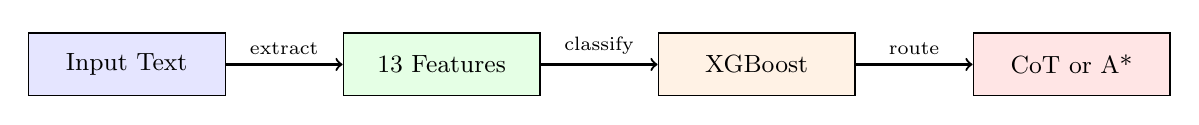
\begin{tikzpicture}[
  box/.style={rectangle, draw, minimum width=2.5cm, minimum height=0.8cm, font=\small},
  arrow/.style={->, thick}
]
\node[box, fill=blue!10] (input) at (0,0) {Input Text};
\node[box, fill=green!10] (feat) at (4,0) {13 Features};
\node[box, fill=orange!10] (clf) at (8,0) {XGBoost};
\node[box, fill=red!10] (out) at (12,0) {CoT or A*};

\draw[arrow] (input) -- (feat) node[midway, above, font=\scriptsize] {extract};
\draw[arrow] (feat) -- (clf) node[midway, above, font=\scriptsize] {classify};
\draw[arrow] (clf) -- (out) node[midway, above, font=\scriptsize] {route};
\end{tikzpicture}
\caption{Topology router pipeline: structural features are extracted from the input text alone (no LLM call), fed to a trained classifier, which outputs the routing decision.}
\label{fig:router_pipeline}
\end{figure}

\section{Experimental Setup}

\subsection{Models}

\begin{itemize}
\item \textbf{LLaMA-3.1-8B-Instruct:} Main backbone for all 8B experiments
\item \textbf{Qwen2-0.5B-Instruct:} Small-scale comparison (tests if search helps weak models)
\item \textbf{Qwen-2.5-14B-Instruct:} Large-scale comparison
\item \textbf{DeepSeek-R1-Distill-Qwen-14B:} Critic/judge model for post-hoc routers
\end{itemize}

All models served locally via Ollama (v0.3.x) or vLLM (v0.4.x).

\subsection{Datasets}

\begin{table}[ht]
\centering
\small
\begin{tabular}{llcc}
\toprule
\textbf{Dataset} & \textbf{Domain} & \textbf{Size} & \textbf{Format} \\
\midrule
StrategyQA & Commonsense QA & 2,290 & Boolean \\
LogicQA & Logical reasoning & 651 & 4-way MC \\
HotpotQA & Multi-hop QA & 500 & Free-form \\
GSM8K & Math (grade school) & 1,319 & Numeric \\
MATH & Math (competition) & 500 & Numeric \\
HumanEval & Code generation & 163 & Function \\
MBPP & Code generation & 500 & Function \\
CodeContests & Algorithmic code & 500 & Function \\
\bottomrule
\end{tabular}
\caption{Dataset summary. We evaluate across three domains (QA, math, code) to test generalization of the topology framework.}
\label{tab:datasets}
\end{table}

\subsection{Hardware and Compute}

All experiments run on a single node with 2$\times$ NVIDIA A100 80GB GPUs. Total compute for the full pipeline: approximately 340 GPU-hours. CoT uses greedy decoding (deterministic); A* uses temperature-based branching. Router training uses 5-fold stratified cross-validation (seed=42).

\subsection{Evaluation Metrics}

\begin{itemize}
\item \textbf{Accuracy:} Exact match for QA/math; functional correctness (pass@1) for code
\item \textbf{Oracle:} Instance-wise best of CoT and A* (upper bound on routing)
\item \textbf{Gap\%:} $\frac{\text{Router} - \text{Best Single}}{\text{Oracle} - \text{Best Single}} \times 100$ (percentage of oracle gap recovered)
\end{itemize}
